\documentclass[11pt]{article}

\usepackage{common}
\usepackage{booktabs}
\title{Practical Write-Up}
\author{Rodney Lafuente\hspace{4cm}Roger Brockett \\ 
lafuentemercado@college.harvard.edu\hspace{1cm}rbrockett@college.harvard.edu}
\date{April 15, 2022}
\begin{document}


\maketitle{}

\section{Part A: Feature Engineering, Baseline Models}

\subsection{Approach}

What did you do? When relevant, provide mathematical descriptions or pseudocode. Credit will be given for:

  \begin{itemize}
  \item PCA:  Describe what the top 500 principal components represent, and how you computed them.
  \item Logistic regression: Describe how the model you trained predicts output probabilities for each class.
  \end{itemize}

\subsection{Results}

This section should report on the following questions: 

\begin{itemize}
\item  What is the \textbf{overall} and \textbf{per-class} classification accuracy of the models that you implemented?
\begin{table}[h]
\centering
\begin{tabular}{llrrr}
    \toprule
    Accuracy &  & Raw Amplitude & Mel Spectogram \\
    \midrule
    \textsc{Overall} & & 0.198 & 0.252 \\
    \textsc{Class 0} & & 0.197 & 0.160 \\
    \textsc{Class 1} & & 0.026 & 0.462 \\
    \textsc{Class 2} & & 0.592 & 0.020 \\
    \textsc{Class 3} & & 0.096 & 0.183 \\
    \textsc{Class 4} & & 0.072 & 0.227 \\
    \textsc{Class 5} & & 0.174 & 0.303 \\
    \textsc{Class 6} & & 0.033 & 0.433 \\
    \textsc{Class 7} & & 0.119 & 0.102 \\
    \textsc{Class 8} & & 0.140 & 0.945 \\
    \textsc{Class 9} & & 0.160 & 0.133 \\
    \bottomrule
\end{tabular}
\caption{\label{tab:rf_results} Accuracies of Logistic Regression models on Raw Amplitude and Mel Spectogram Data.}
\end{table}
\end{itemize}


\begin{figure}[h]
    \centering
    \begin{minipage}{0.45\textwidth}
        \centering
        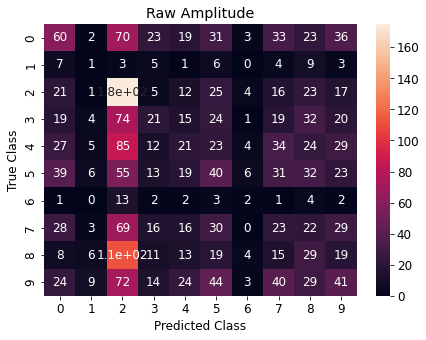
\includegraphics[width=1\textwidth]{amp_lr_cfm} % first figure itself
        \caption{Confusion Matrix of Logistic Regression on Raw Amplitude Data}
    \end{minipage}\hfill
    \begin{minipage}{0.45\textwidth}
        \centering
        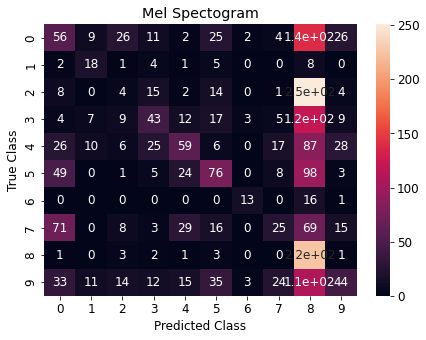
\includegraphics[width=1\textwidth]{mel_lr_cfm} % second figure itself
        \caption{Confusion Matrix of Logistic Regression on Mel Spectogram Data}
    \end{minipage}
\end{figure}


\subsection{Discussion}

This section should report on the following questions: 

\begin{itemize}
  \item Why do you hypothesize one feature representation performed better than the other?  
  \item Why might have asked you to perform PCA first, and what is the impact of that choice?
  \end{itemize}

\section{Part B: More Modeling}

\subsection{First Step}

\subsubsection{Approach}

What did you do? Credit will be given for:

  \begin{itemize}
  \item Provide mathematical descriptions or pseudocode to help us understand how the models you tried make predictions and are trained.
  \end{itemize}

\subsubsection{Results}
This section should report on the following questions: 

\begin{itemize}
\item  What is the overall and per-class classification accuracy of the models that you implemented?
    \begin{table}[h]
    \centering
    \begin{tabular}{llrrr}
        \toprule
        Accuracy &  & Raw Amplitude & Mel Spectogram \\
        \midrule
        \textsc{Overall} & & 0.248 & 0.334 \\
        \textsc{Class 0} & & 0.230 & 0.280 \\
        \textsc{Class 1} & & 0.000 & 0.256 \\
        \textsc{Class 2} & & 0.746 & 0.211 \\
        \textsc{Class 3} & & 0.035 & 0.424 \\
        \textsc{Class 4} & & 0.110 & 0.216 \\
        \textsc{Class 5} & & 0.390 & 0.375 \\
        \textsc{Class 6} & & 0.033 & 0.167 \\
        \textsc{Class 7} & & 0.102 & 0.356 \\
        \textsc{Class 8} & & 0.212 & 0.441 \\
        \textsc{Class 9} & & 0.127 & 0.437 \\
        \bottomrule
    \end{tabular}
    \caption{\label{tab:lr_results} Accuracies of Random Forest Classifier models on Raw Amplitude and Mel Spectogram Data.}
    \end{table}

    \begin{figure}[h!]
        \centering
        \begin{minipage}{0.45\textwidth}
            \centering
            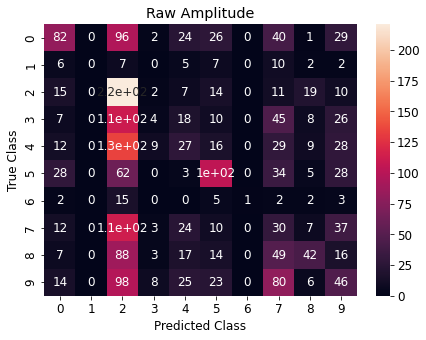
\includegraphics[width=1\textwidth]{amp_rf_cfm} % first figure itself
            \caption{Confusion Matrix of Random Forest Classifier on Raw Amplitude Data}
        \end{minipage}\hfill
        \begin{minipage}{0.45\textwidth}
            \centering
            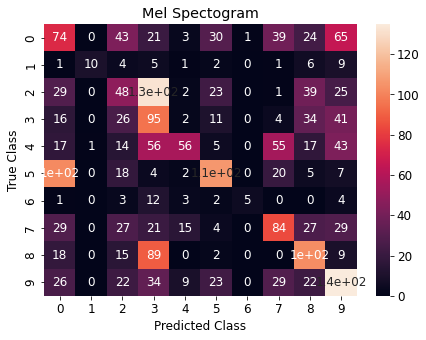
\includegraphics[width=1\textwidth]{mel_rf_cfm} % second figure itself
            \caption{Confusion Matrix of Random Forest Classifier on Mel Spectogram Data}
        \end{minipage}
    \end{figure}
\end{itemize}



\subsubsection{Discussion}
Compare your results to the logistic regression models in Part A and discuss what your results imply about the task.


\subsection{Hyperparameter Tuning and Validation}

\subsubsection{Approach}
What did you do? Credit will be given for:

  \begin{itemize}
  \item Making tuning and configuration decisions using thoughtful experimentation.  
    How did you perform your hyperparameter search, and what hyperparameters did you search over?
  \end{itemize}

\subsubsection{Results}
Present your results of your hyperparameter search in a way that best reflects how to communicate your conclusions.

\begin{itemize}
    \item RFC: The results from the hyperparameter grid search on Random Forest Classifiers showed...
    \begin{table}[h]
    \centering
    \begin{tabular}{llrrr}
        \toprule
        \# Estimators & & Raw Amplitude & Mel Spectogram & Overall Rank \\
        \midrule
        \textsc{360} & & 0.235 & 0.423 & 5 \\
        \textsc{400} & & 0.235 & 0.428 & 3 \\
        \textsc{440} & & 0.238 & 0.424 & 4 \\
        \textsc{480} & & 0.240 & 0.426 & 1 \\
        \textsc{520} & & 0.242 & 0.424 & 1 \\
        \bottomrule
    \end{tabular}
    \caption{\label{tab:rf_search_results} Accuracies of Random Forest Models of Varying Estimator Counts}
    \end{table}
    
    \item SVM: The results on ...
    \begin{table}[h]
    \centering
    \begin{tabular}{llrrr}
        \toprule
        C Value & & Raw Amplitude & Mel Spectogram & Overall Rank \\
        \midrule
        \textsc{0.001} & & 0.123 & 0.123 & 5 \\
        \textsc{0.01}  & & 0.141 & 0.123 & 4 \\
        \textsc{0.1}   & & 0.160 & 0.185 & 3 \\
        \textsc{1}     & & 0.175 & 0.267 & 2 \\
        \textsc{10}    & & 0.188 & 0.322 & 1 \\
        \bottomrule
    \end{tabular}
    \caption{\label{tab:svm_search_results} Accuracies of Support Vector Machine models of Varying C Values}
    \end{table}

\end{itemize}


\subsubsection{Discussion}

Why do you expect the tuned models to perform better than the baseline models and the model used in First Step? Discuss your validation strategy and your conclusions.

% \section{Optional Exploration, Part C: Explore some more!}
% \subsection{Approach}

% What did you do? Credit will be given for:
%   \begin{itemize}
%   \item Diving deeply into all of the model classes and/or pre-processing algorithms that you tried (rather than just trying off-the-shelf tools with default settings).  When relevant, provide mathematical descriptions or pseudocode to help us understand how the models you tried make predictions and are trained. 
%   \end{itemize}
  

% \subsection{Results}

% Describe your results in a way that is appropriate for the experiments that you ran.

% \subsection{Discussion}
% Credit will be given for:

%   \begin{itemize}
%   \item Explaining the your reasoning for why you sequentially chose to
%     try the approaches you did (i.e. what was it about your initial
%     approach that made you try the next change?).  
%   \item Explaining the results.  Did the adaptations you tried improve
%     the results?  \textbf{Why or why not?}  Did you do additional tests to
%     determine if your reasoning was correct?  
%   \end{itemize}
 

\end{document}